

\tikzset{every picture/.style={line width=0.75pt}} %set default line width to 0.75pt        

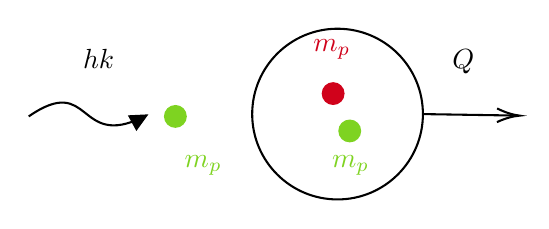
\begin{tikzpicture}[x=0.75pt,y=0.75pt,yscale=-1,xscale=1]
%uncomment if require: \path (0,408); %set diagram left start at 0, and has height of 408

%Curve Lines [id:da5989822671081096] 
\draw    (50.33,146) .. controls (80.88,124.88) and (73.41,162.06) .. (105.46,146.32) ;
\draw [shift={(108,145)}, rotate = 151.5] [fill={rgb, 255:red, 0; green, 0; blue, 0 }  ][line width=0.08]  [draw opacity=0] (8.93,-4.29) -- (0,0) -- (8.93,4.29) -- cycle    ;
%Flowchart: Connector [id:dp08119567255108817] 
\draw  [color={rgb, 255:red, 126; green, 211; blue, 33 }  ,draw opacity=1 ][fill={rgb, 255:red, 126; green, 211; blue, 33 }  ,fill opacity=1 ] (116,146) .. controls (116,143.24) and (118.24,141) .. (121,141) .. controls (123.76,141) and (126,143.24) .. (126,146) .. controls (126,148.76) and (123.76,151) .. (121,151) .. controls (118.24,151) and (116,148.76) .. (116,146) -- cycle ;
%Flowchart: Connector [id:dp04975844425187159] 
\draw  [color={rgb, 255:red, 208; green, 2; blue, 27 }  ,draw opacity=1 ][fill={rgb, 255:red, 208; green, 2; blue, 27 }  ,fill opacity=1 ] (192,135) .. controls (192,132.24) and (194.24,130) .. (197,130) .. controls (199.76,130) and (202,132.24) .. (202,135) .. controls (202,137.76) and (199.76,140) .. (197,140) .. controls (194.24,140) and (192,137.76) .. (192,135) -- cycle ;
%Flowchart: Connector [id:dp029263123361565446] 
\draw  [color={rgb, 255:red, 126; green, 211; blue, 33 }  ,draw opacity=1 ][fill={rgb, 255:red, 126; green, 211; blue, 33 }  ,fill opacity=1 ] (200,153) .. controls (200,150.24) and (202.24,148) .. (205,148) .. controls (207.76,148) and (210,150.24) .. (210,153) .. controls (210,155.76) and (207.76,158) .. (205,158) .. controls (202.24,158) and (200,155.76) .. (200,153) -- cycle ;
%Shape: Circle [id:dp6718718103888768] 
\draw   (158,144.88) .. controls (158,122.16) and (176.41,103.75) .. (199.12,103.75) .. controls (221.84,103.75) and (240.25,122.16) .. (240.25,144.88) .. controls (240.25,167.59) and (221.84,186) .. (199.12,186) .. controls (176.41,186) and (158,167.59) .. (158,144.88) -- cycle ;
%Straight Lines [id:da24501455375525605] 
\draw    (240.25,144.88) -- (284.89,145.59) ;
\draw [shift={(286.89,145.63)}, rotate = 180.92] [color={rgb, 255:red, 0; green, 0; blue, 0 }  ][line width=0.75]    (10.93,-3.29) .. controls (6.95,-1.4) and (3.31,-0.3) .. (0,0) .. controls (3.31,0.3) and (6.95,1.4) .. (10.93,3.29)   ;

% Text Node
\draw (75,112.4) node [anchor=north west][inner sep=0.75pt]    {$hk$};
% Text Node
\draw (124,163.4) node [anchor=north west][inner sep=0.75pt]  [color={rgb, 255:red, 126; green, 211; blue, 33 }  ,opacity=1 ]  {$m_{p}$};
% Text Node
\draw (195,163.4) node [anchor=north west][inner sep=0.75pt]  [color={rgb, 255:red, 126; green, 211; blue, 33 }  ,opacity=1 ]  {$m_{p}$};
% Text Node
\draw (186,107.4) node [anchor=north west][inner sep=0.75pt]  [color={rgb, 255:red, 208; green, 2; blue, 27 }  ,opacity=1 ]  {$m_{p}$};
% Text Node
\draw (253,112.4) node [anchor=north west][inner sep=0.75pt]    {$Q$};


\end{tikzpicture}